\subsection{RQ2. Comparative study on Java Dataset}


\begin{table}[t]
	\caption{RQ1. Comparison on C\# Dataset ($Accuracy^c$\%)}
	\vspace{-0.1in}
	\begin{center}
		\footnotesize
		\tabcolsep 4pt
		\renewcommand{\arraystretch}{1} \begin{tabular}{p{0.5cm}<{\centering}|p{1.2cm}<{\centering}|p{1.2cm}<{\centering}|p{1.2cm}<{\centering}|p{1.2cm}<{\centering}|p{1.2cm}<{\centering}}
			
			\hline
			          & Base-1 & Base-2  & Base-3 & SmartCommit & \bf {\tool}\\
			\hline
			SB   & 14 & 23 & 21 & 29 & 32\\
			ES   & 19 & 22 & 27 & 34 & 36\\
			RJ   & 18 & 28 & 24 & 31 & 33\\
			GU   & 21 & 31 & 25 & 33 & 37\\
			RE   & 22 & 24 & 19 & 29 & 34\\
			DU   & 15 & 19 & 18 & 24 & 29\\
			GH   & 22 & 27 & 24 & 33 & 35\\
			ZX   & 21 & 29 & 20 & 34 & 38\\
			DR   & 17 & 29 & 18 & 32 & 34\\
			EB   & 13 & 22 & 21 & 27 & 31\\
			\hline
			OA   &  17  & 25 &  23 & 30 & {\bf 34} \\
			\hline
		\end{tabular}
		\label{RQ2-result-1}
	SB: spring-boot, ES: elasticsearch, RJ: RxJava, GU:guava, RE: retrofit, DU: dubbo, GH: ghidra, ZX: zxing, DR: druid, EB: EventBus, OA: Overall
	\end{center}
\end{table}


\begin{figure}
	\centering
	\begin{subfigure}{0.235\textwidth}
	\centering
	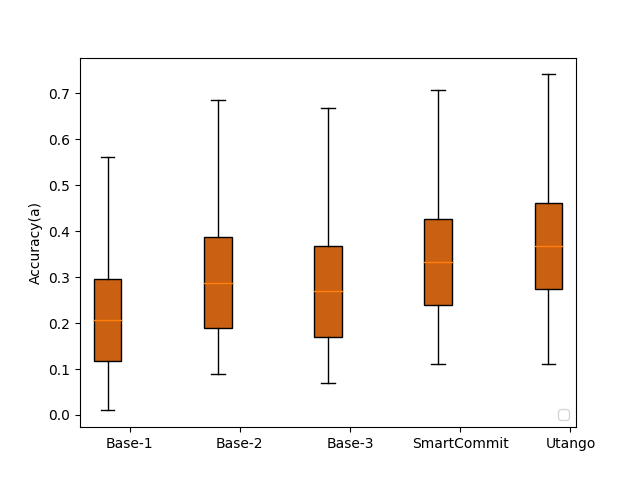
\includegraphics[width=1.6in]{figures/RQ_2_1.png}
	\vspace{-8pt}
	\caption{Boxplots for the Results in Table~\ref{RQ2-result-1}}
	\label{RQ2-result-2}
	\end{subfigure}
\hfill
	\begin{subfigure}{0.225\textwidth}
		\centering
		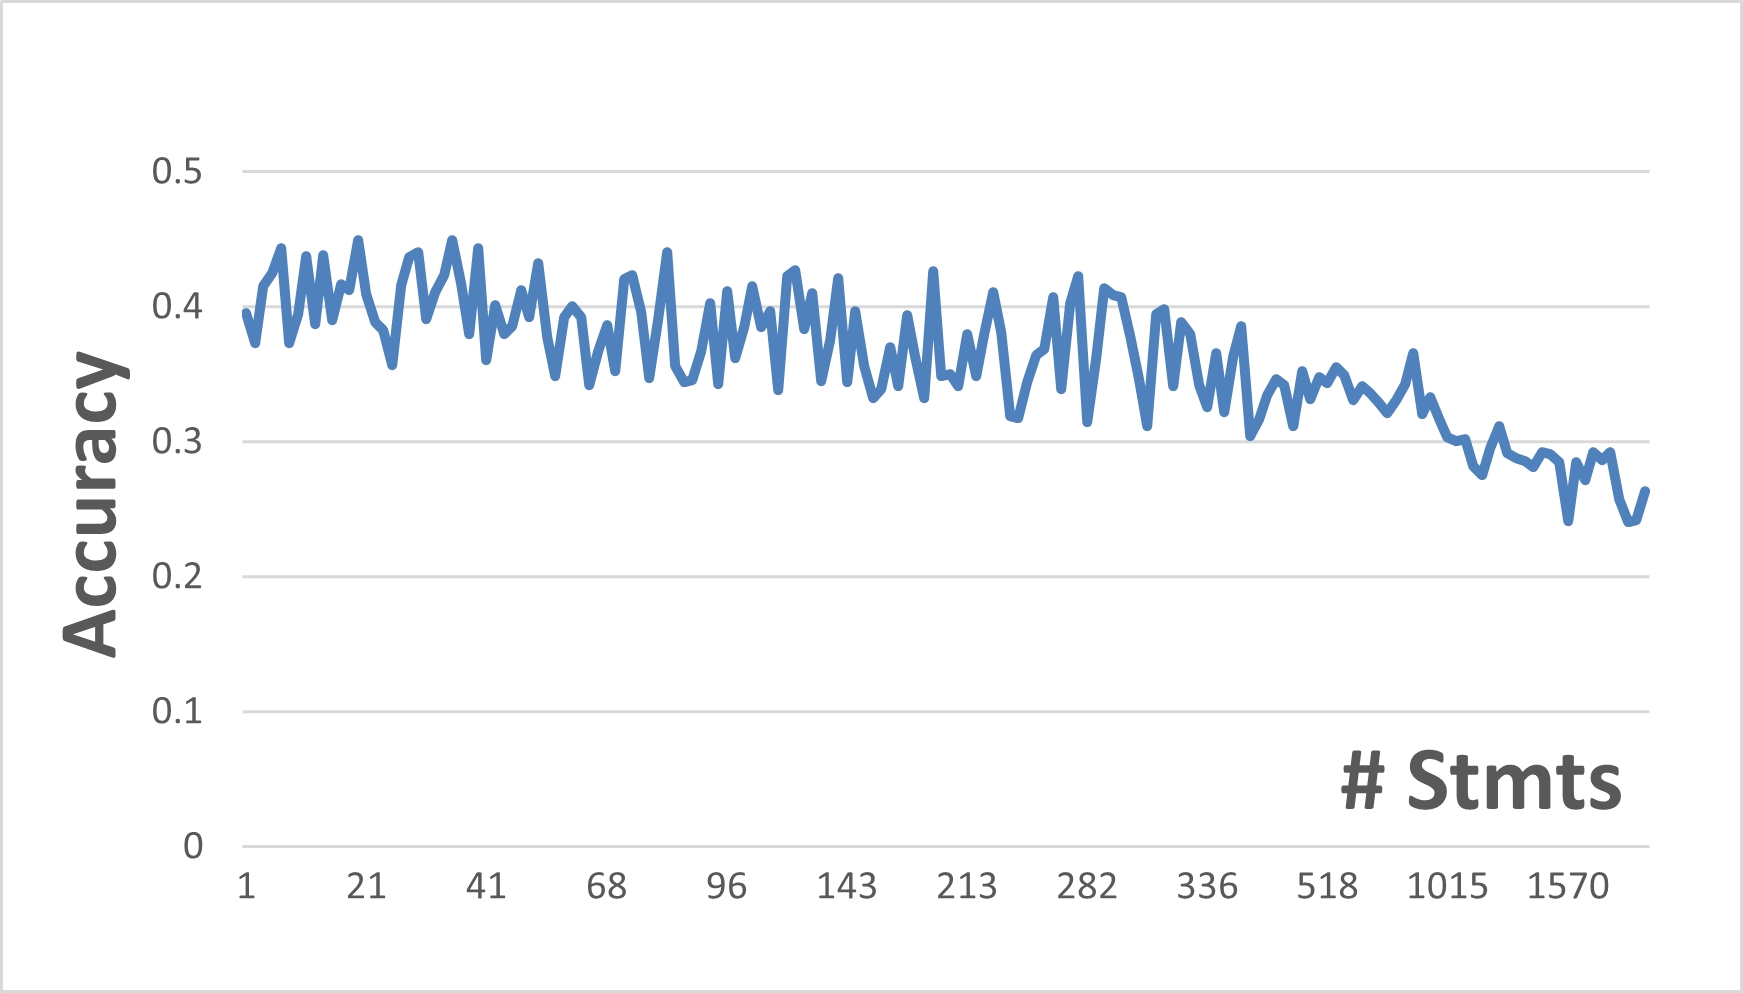
\includegraphics[width=1.7in]{figures/accuracy-concerns-java.png}
		\vspace{-8pt}
		\caption{Accuracy for Concerns with Diff. Numbers of Stmts}
		\label{RQ2-result-3}
	\end{subfigure}
	\label{RQ2-result-4}
	\vspace{-12pt}
	\caption{Java Dataset Results Analysis}
\end{figure}

{\color{red}{ 1--22 changed statements: 37\%--45\%. Lowest: 24\%
	
100\% correct: \tool: 116, SmartCommit: 109, Overlapping: 21}}